\chapter{RESULTADOS E VALIDAÇÃO}
\label{cap:resultados}

A validação usou testes automatizados que exercitam o sistema como um usuário, contra o SQL Server real e a partir de uma base zerada \cite{pressman2021}. Os testes do Web e da API são executados por um \textit{script} (testes/rodar.sh) que recria a base a cada execução. A Tabela~\ref{tab:testes} resume os conjuntos de testes e seus resultados.

\begin{table}[htbp]
\centering
\caption{Testes automatizados e resultados}
\label{tab:testes}
\footnotesize
\begin{tabular}{|p{3.6cm}|p{7.6cm}|c|}
\hline
\textbf{Conjunto} & \textbf{O que verifica} & \textbf{Resultado} \\ \hline
Web (navegação HTTP) & Login e perfis, cadastros, filtros de pedidos, as sete combinações de regras do carregamento (RN08, RN09, RN17, RN18, RN19), cancelamento, aprovação de entrada e rastreio & 36 de 36 \\ \hline
API (ciclo completo) & Token por perfil, respostas 401 e 403, entrada com e sem diferença (RN01--RN03), carregamento (RN10, RN11), saída, entregas (RN13), volta e encerramento (RF16) e retorno (RN14) & 48 de 48 \\ \hline
Aplicativo (unidade) & Conversão do JSON e tratamento de erros do cliente HTTP & 8 de 8 \\ \hline
Aplicativo (ponta a ponta) & Ciclo completo de um pedido pelas telas do aplicativo, falando com a API real & aprovado \\ \hline
Banco de dados & As duas \textit{procedures} e os dois \textit{triggers} executados diretamente no SQL Server & aprovado \\ \hline
\end{tabular}
\fonte{Elaborado pelo autor (2026)}
\end{table}

O teste de ponta a ponta do aplicativo percorre o ciclo de vida do pedido da Figura~\ref{fig:status}: entrada da nota, bipagem das vinte caixas de dois pedidos, saída recusada e depois liberada, uma entrega e uma não entrega com motivo, volta, encerramento e retorno das caixas, com o pedido voltando para Aberto.

\begin{figure}[htbp]
\centering
\caption{Ciclo de vida do pedido validado pelos testes}
\label{fig:status}
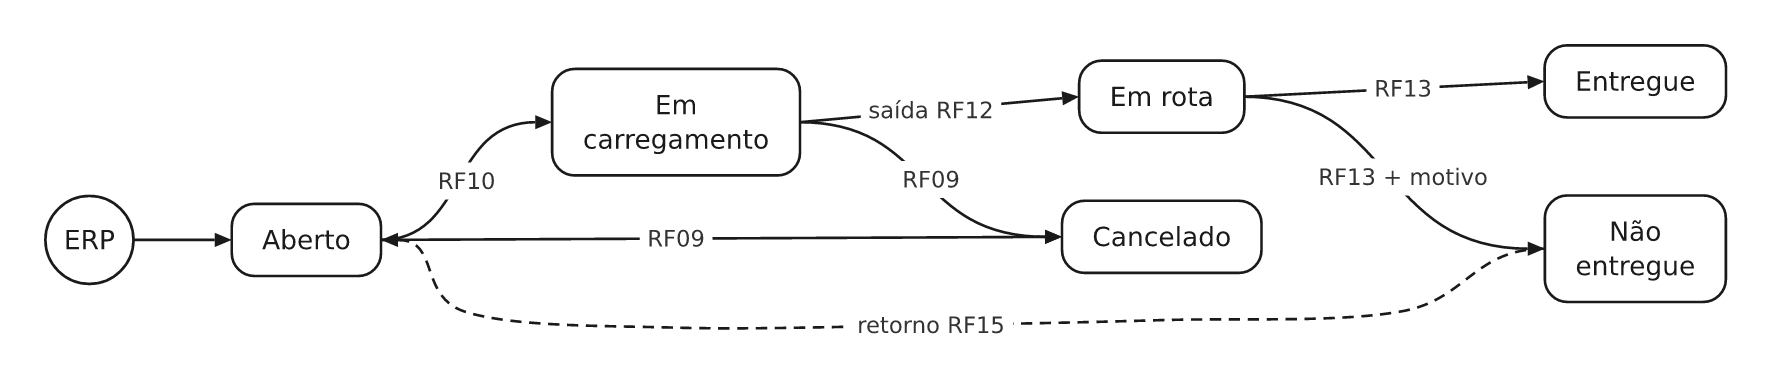
\includegraphics{figuras/status_pedido.png}
\fonte{Elaborado pelo autor (2026)}
\end{figure}

Assim, os dezenove requisitos e as dezenove regras estão implementados e testados, cobrindo os problemas P1 a P6 do Capítulo 2: cada leitura gera histórico, o pedido tem status até a entrega, a caixa errada é recusada, a portaria só libera carga completa, a frota é respeitada e o retorno reabre o pedido.

As limitações são a dependência de conexão no momento da leitura, a integração com o ERP feita por carga inicial e a nuvem e a esteira de CI/CD apenas projetadas; todas estão no \textit{backlog} como histórias futuras.
